\documentclass[]{report}
\usepackage{hyperref}
\usepackage{amsmath}
\usepackage{graphicx}
\usepackage[]{mcode}
\usepackage{multirow}

\hypersetup{colorlinks=true, linkcolor=black, urlcolor=blue}
% Title Page
\title{Project: Image Analysis 2015/2016\\Anomaly Detection for Crop Monitoring:\\ Report}

\author{Stefano Cerri 849945}


\begin{document}
\maketitle
\tableofcontents
\listoffigures

\chapter{Scope}

\section{Problem}

One of the most important tasks to be addressed in intelligent farms is the crop monitoring. Computer Vision and Machine Learning algorithms are typically combined to analyze and classify images acquired by autonomous robots that monitor the growth of crops, and in particular, to discriminate crops (i.e. the good plants) from weeds (any undesirable or unwanted plant growing wild, especially those that takes food or nourishment from crops). Crop/weed discrimination are often tacked as an image-classification problem.


\section{Dataset}

The dataset used in this project is the CWFID dataset\footnote{https://github.com/cwfid/dataset}. It comprises field images, vegetation segmentation masks and crop/weed plant type annotations. The paper\footnote{see Appendix$\rightarrow  $Reference document} provides details, e.g. on the field setting, acquisition conditions, image and ground truth data format.
All images were acquired with the autonomous field robot Bonirob in an organic carrot farm while the carrot plants were in early true leaf growth stage.

\section{Assignment}

The assignment is to create a Convolutional Neural Network, using deep learning, that classificates the images in crop,weed or ground. 

\chapter{Extract patches from the dataset}

This work was done by two collegues,Jorge Carpio Lopez de Castro and  Andrea Luigi Edoardo Caielli, that work on the same project. 
The script creates a dataset of patches (with dimension $ 51\times51\times3 $). A patch is a sub-region of an image that has a particular property. In our case there are three types of patches: crop patches, weed patches and ground patches. The result of the script is a dataset composed of:

\begin{itemize}
	\item \textbf{3000 training patches} : 1000 crop, 1000 weed, 1000 ground 
	\item \textbf{3000 testing patches} : 1000 crop, 1000 weed, 1000 ground
\end{itemize}

Here some examples of patches:

\begin{figure}[!htb]
\minipage{0.32\textwidth}
  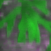
\includegraphics[width=\linewidth]{crop.png}
  \caption{crop patch}\label{fig:crop sample}
\endminipage\hfill
\minipage{0.32\textwidth}
  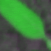
\includegraphics[width=\linewidth]{weed.png}
  \caption{weed patch}\label{fig:weed sample}
\endminipage\hfill
\minipage{0.32\textwidth}%
  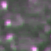
\includegraphics[width=\linewidth]{ground.png}
  \caption{ground patch}\label{fig:ground sample}
\endminipage
\end{figure}



\chapter{Training the network}

\section{MatConvNet library}

To perform the given assignment I donloaded and installed MatConvNet library\footnote{http://www.vlfeat.org/matconvnet/}. Note that in order to use some functionalities of the library, such as using GPU acceleration, it has some requirements\footnote{http://www.vlfeat.org/matconvnet/gpu/}.
There is also a manual\footnote{http://www.vlfeat.org/matconvnet/matconvnet-manual.pdf} that explains all the blocks of a CNN both from the "mathematical" and "code function" view. The configuration that I used was:

\begin{itemize}

	\item MatConvNet 1.0-beta18
	\item Matlab 2016a	
	
\end{itemize}  

\section{What is a Convolutional Neural Network?}

CNN is a type of feed-forward artificial neural network in which the connectivity pattern between its neurons is inspired by the organization of the animal visual cortex, whose individual neurons are arranged in such a way that they respond to overlapping regions tiling the visual field.It consist of multiple layers of small neuron collections which process portions of the input image, called receptive fields. The outputs of these collections are then tiled so that their input regions overlap, to obtain a better representation of the original image; this is repeated for every such layer. A more detailed description of the layer of a Convolutional Neural Network can be found in the next section.

\begin{figure}[h]
	\begin{center}
		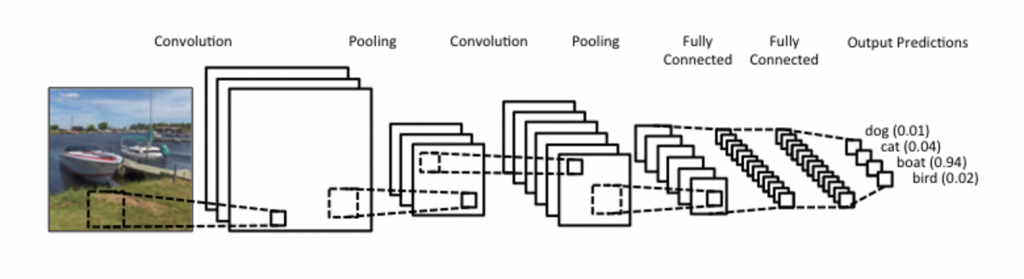
\includegraphics[scale=0.3]{CNN.png}
		\caption{Example of a Convolutional Neural Network}
		\label{fig:CNN}
	\end{center}
\end{figure}
\newpage
\section{Build the architecture of the network}

\subsection{Typical layer of a CNN}

The typical layer of a Convolutional Neural Network are:

\begin{itemize}

\item \textbf{Convolutional layer}:it is the core building block of a Convolutional Network, and its output volume can be interpreted as holding neurons arranged in a 3D volume.The CONV layer's parameters consist of a set of learnable filters. Every filter is small spatially (along width and height), but extends through the full depth of the input volume. During the forward pass, we slide (more precisely, convolve) each filter across the width and height of the input volume, producing a 2-dimensional activation map of that filter. As we slide the filter, across the input, we are computing the dot product between the entries of the filter and the input. Intuitively, the network will learn filters that activate when they see some specific type of feature at some spatial position in the input. Stacking these activation maps for all filters along the depth dimension forms the full output volume. Every entry in the output volume can thus also be interpreted as an output of a neuron that looks at only a small region in the input and shares parameters with neurons in the same activation map (since these numbers all result from applying the same filter).Three hyperparameters control the size of the output volume: the \textbf{depth}, \textbf{stride} and \textbf{zero-padding}

\item \textbf{Pooling Layer}:it is common to periodically insert a Pooling layer in-between successive Conv layers in a ConvNet architecture. Its function is to progressively reduce the spatial size of the representation to reduce the amount of parameters and computation in the network, and hence to also control overfitting. The Pooling Layer operates independently on every depth slice of the input and resizes it spatially, using the MAX operation. The most common form is a pooling layer with filters of size 2x2 applied with a stride of 2 downsamples every depth slice in the input by 2 along both width and height, discarding 75\% of the activations. Every MAX operation would in this case be taking a max over 4 numbers (little 2x2 region in some depth slice). The depth dimension remains unchanged

\item \textbf{Fully-connected layer}:neurons in a fully connected layer have full connections to all activations in the previous layer. Their activations can hence be computed with a matrix multiplication followed by a bias offset.In other libraries,fully connected blocks or layers are linear functions where each output dimension depends on all the input dimensions.MatConvNet does not distinguish between fully connected layers and convolutional blocks

\item \textbf{ReLu}:the rectified linear unit will apply an elementwise activation function, such as the $ f(x) = max(0,x) $ thresholding at zero. This leaves the size of the volume unchanged 

\item \textbf{SoftMax}: Soft Max is a loss functionakes the score compete through the normalization
factor.Softmax can be seen as the combination of an activation function
(exponential) and a normalization operator

\end{itemize}


\subsection{Typical architecture}

The most common form of a ConvNet architecture stacks a few CONV-RELU layers, follows them with POOL layers, and repeats this pattern until the image has been merged spatially to a small size. At some point, it is common to transition to fully-connected layers. The last fully-connected layer holds the output, such as the class scores. In other words, the most common ConvNet architecture follows the pattern:

$INPUT\rightarrow [[CONV\rightarrow RELU]*N\rightarrow POOL?]*M\rightarrow[FC\rightarrow RELU]*K\rightarrow FC \rightarrow LOSS $

where the $ * $ indicates repetition, and the POOL? indicates an optional pooling layer. Moreover, $ N>=0 $ (and usually $ N<=3 $), $M >= 0$,$ K >= 0$ (and usually $ K < 3$).

\subsection{Selected architectures}

I selected different network architectures for comparing it, after the training, with the testing set. The architectures are:

\begin{enumerate}

\item $ INPUT \rightarrow [CONV \rightarrow RELU \rightarrow POOL]*2 \rightarrow FC \rightarrow RELU \rightarrow FC \rightarrow LOSS $ 

\item $ INPUT \rightarrow [CONV \rightarrow RELU \rightarrow POOL]*3 \rightarrow FC \rightarrow LOSS $ 

\item $ INPUT \rightarrow [CONV \rightarrow RELU \rightarrow POOL]*4 \rightarrow FC \rightarrow LOSS $ 

\item $ INPUT \rightarrow [CONV \rightarrow RELU \rightarrow POOL]*3 \rightarrow FC \rightarrow LOSS $ 

\item $ INPUT \rightarrow [CONV \rightarrow RELU \rightarrow POOL]*3 \rightarrow FC \rightarrow RELU \rightarrow FC \rightarrow LOSS $ 

\item $ INPUT \rightarrow [CONV \rightarrow RELU \rightarrow POOL]*3 \rightarrow [FC \rightarrow RELU]*2 \rightarrow FC \rightarrow LOSS $ 

\end{enumerate}


\section{Train the network}

\subsection{Create a validation set}

In order to avoid overfitting I split the testing set into two sets; a validation test and a test set.The validetion set can be seen as a set of examples used to tune the parameters of the classifier. The final dataset is composed by:

\begin{itemize}

	\item \textbf{training set}: 3000 patches: 1000 crop patches, 1000 weed patches, 1000 ground patches
	\item \textbf{validation set}: 1500 patches: 500 crop patches, 500 weed patches, 500 ground patches
	\item \textbf{testing set}: 1500 patches: 500 crop patches, 500 weed patches, 500 ground patches
	
\end{itemize}

\subsection{Stochastic gradient descent with momentum}

To train the network I used stochastich gradient descent with momentum. Stochastic gradient descent (often shortened in SGD) is a stochastic approximation of the gradient descent optimization method for minimizing an objective function that is written as a sum of differentiable functions. The problem of minimizing an objective function can be describe as:

\begin{center}

	$ Q(w)= \sum\limits_{i=1}^n Q_{i}(w) $

\end{center}

where the parameter $  $ which minimizes $ Q(w) $ is to be estimated. Each summand function $ Q_{i} $ is typically associated with the $ i-th $ observation in the data set (used for training). 
Stochastic gradient descent with momentum remembers the update $ \Delta w $ at each iteration, and determines the next update as a convex combination of the gradient and the previous update

\begin{center}

	$ \Delta w:= \eta \bigtriangledown  Q_{i}(w) + \alpha \Delta w $\\
	$ w := w+ \Delta w $

\end{center}

where $ \eta $ is the learning rate.

\subsection{Function used}
The function cnn\textunderscore train.m can be used with different datasets and tasks by providing a suitable getBatch function (implemented in  cnn\textunderscore cwfid.m). The function automatically restarts after each training epoch by checkpointing. The function supports training on CPU or on one or more GPUs (specify the list of GPU IDs in the `gpus` option). Multi-GPU support is relatively primitive but sufficient to obtain a noticable speedup.

\subsection{Results of the training}
Here are the 6 networks training graph. On the left side there is the objective function and on the right side there is the error function.

\begin{figure}[h]
	\begin{center}
		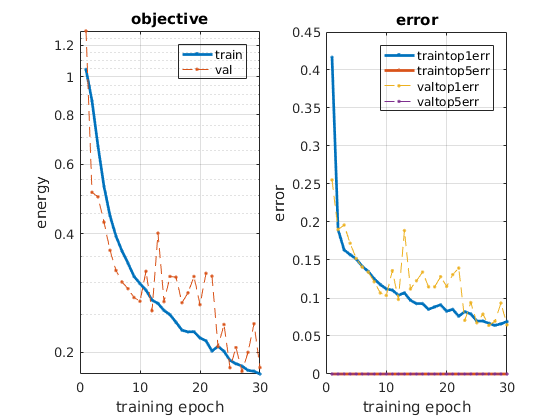
\includegraphics[scale=0.5]{init_1.png}
		\caption{network 1 training}
		\label{fig:training1}
	\end{center}
\end{figure}

\begin{figure}[h]
	\begin{center}
		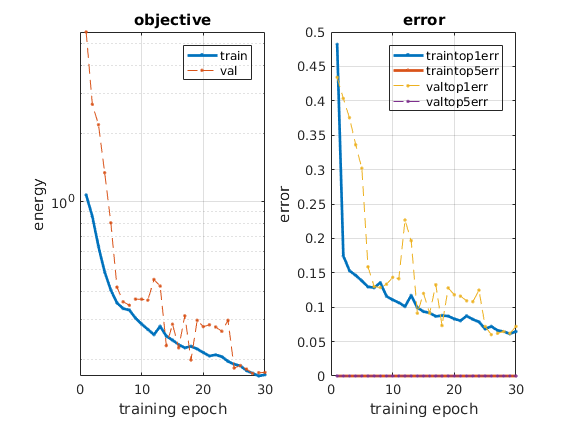
\includegraphics[scale=0.5]{init_2.png}
		\caption{network 2 training}
		\label{fig:training2}
	\end{center}
\end{figure}

\begin{figure}[h]
	\begin{center}
		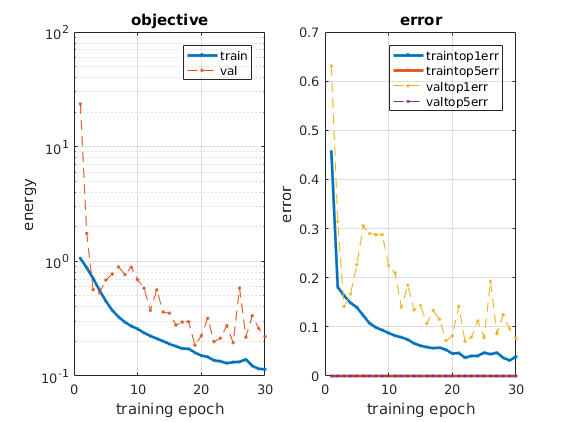
\includegraphics[scale=0.5]{init_3.png}
		\caption{network 3 training}
		\label{fig:training3}
	\end{center}
\end{figure}

\begin{figure}[h]
	\begin{center}
		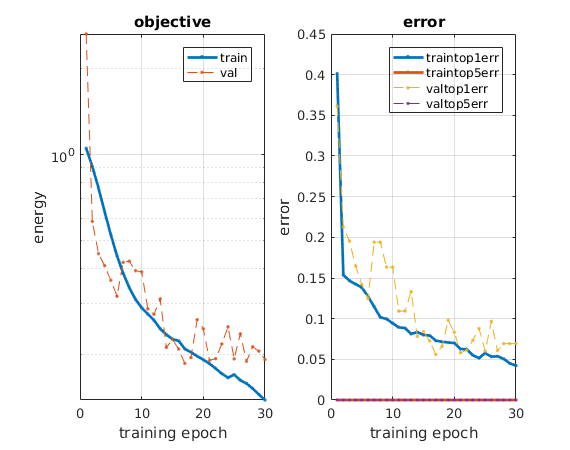
\includegraphics[scale=0.5]{init_4.png}
		\caption{network 4 training}
		\label{fig:training4}
	\end{center}
\end{figure}

\begin{figure}[h]
	\begin{center}
		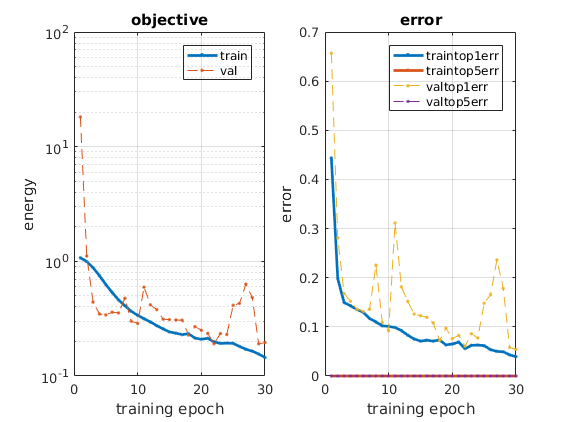
\includegraphics[scale=0.5]{init_5.png}
		\caption{network 5 training}
		\label{fig:training5}
	\end{center}
\end{figure}

\begin{figure}[h]
	\begin{center}
		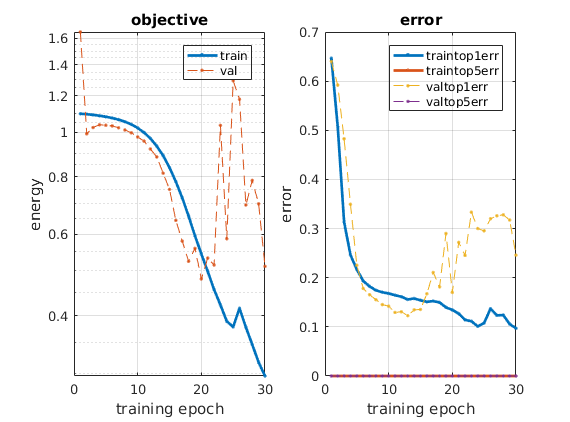
\includegraphics[scale=0.5]{init_6.png}
		\caption{network 6 training}
		\label{fig:training6}
	\end{center}
\end{figure}

\chapter{Evaluate the network}

\section{Compute the accuracy of each network}

In order to evaluate the network I calculate the accuracy. The accuracy can be computed as:

\begin{center}

	$ ACC= \frac{TP+TN}{TP+TN+FP+FN} $

\end{center}

where $ TP = $ true positive , $ TN =$ true negative , $ FP =$ false positive  and $ FN =$ false negative 


\begin{table}[h]
\centering

\begin{tabular}{|c|c|c|c|c|}
 \hline
 \textbf{Network} & \textbf{Accuracy} & \textbf{Accuracy Crop} & \textbf{Accuracy Ground} & \textbf{Accuracy Weed} \\ \hline
 1 & 94,00\% & 92,80\%  & 99,80\%  & 89,40\%  \\ \hline
 2 & 94,07\% & 95,60\%  & 99,80\%  & 86,80\%  \\ \hline
 3 & 92,53\% & 92,20\%  & 99,80\%  & 85,60\%  \\ \hline
 4 & 94,13\% & 93,00\%  & 99,80\%  & 89,60\%  \\ \hline
 \textbf{5} & \textbf{94,20\%} & \textbf{94,00\%}  & \textbf{99,80\%}  & \textbf{88,80\%}  \\ \hline
 6 & 92,33\% & 93,60\%  & 99,80\%  & 83,60\%  \\ \hline
\end{tabular}
\end{table}

\begin{figure}[h]
	\begin{center}
		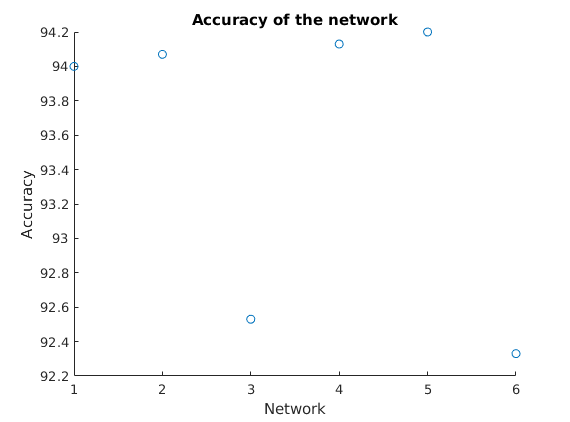
\includegraphics[scale=0.4]{accuracy.png}
		\caption{accuracy of the networks}
		\label{fig:accuracyNetworks}
	\end{center}
\end{figure}

\newpage
The network that has the highest accuracy is \textbf{network 5}. From now on I will discuss and talk about network 5 only because it has the best performance and it is the one that I used for the next step. 

\section{Changing the number of maps of each convolutional filter}

Once the network has been selected I tried to change the number of maps of each convolutional filter in order to increase the accuracy. Here are some combination of number of maps that I used and the correspondent accuracy.

\begin{table} [h]
\begin{center}
\begin{tabular}{|c|c|c|c|c|}
 \hline
 \textbf{Filter 1} & \textbf{Filter 2} & \textbf{Filter 3} & \textbf{Filter 4} & \textbf{Accuracy} \\ \hline
 10 & 20 & 40  & 80  & 94,20\%  \\ \hline
 15 & 30 & 60  & 120  & 92,60\%  \\ \hline
 \textbf{8} & \textbf{16} & \textbf{32}  & \textbf{64}  & \textbf{94,33\%}  \\ \hline
 7 & 14 & 28  & 56  & 93,73\%  \\ \hline
 9 & 18 & 36  & 72  & 93,20\%  \\ \hline
 12 & 24 & 48  & 96  & 92,53\%  \\ \hline
 
\end{tabular}
\end{center} 
\end{table}
 
\begin{figure}[h]
	\begin{center}
		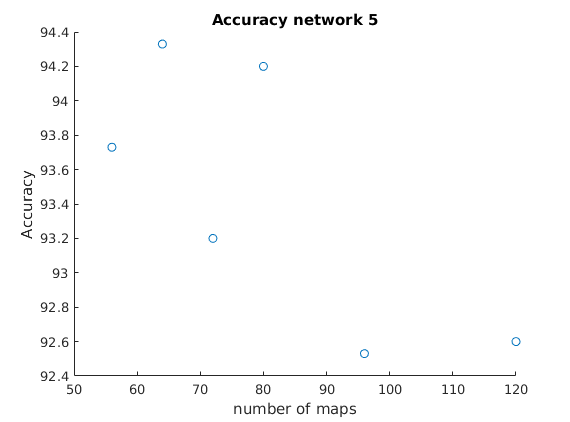
\includegraphics[scale=0.4]{maps_accuracy.png}
		\caption{accuracy VS number of maps; only the number of maps of the last filter layer is plotted in the graph}
		\label{fig:accuracyMaps}
	\end{center}
\end{figure}

\newpage   
This is the training graph with a better combination of number of maps. This configuration is the final one that I used for the given assignment and has a global accuracy of \textbf{94,33\%} \textbf{94,20\%} for crop \textbf{99,80\%} for ground and \textbf{89,00\%} for weed.

\begin{figure}[h]
	\begin{center}
		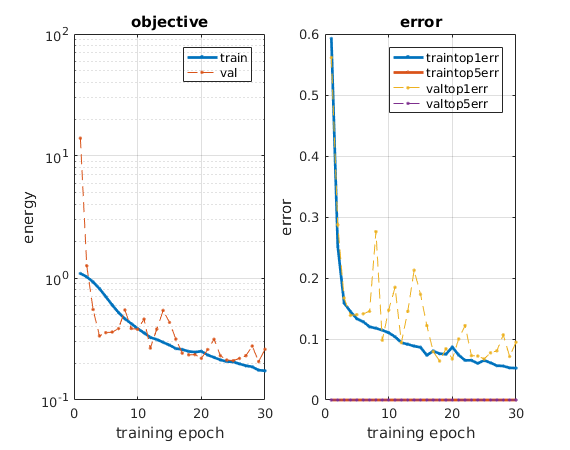
\includegraphics[scale=0.5]{final.png}
		\caption{final training}
		\label{fig:FinalTraining}
	\end{center}
\end{figure}
\newpage

\section{Calculate Confusion Matrix}

In order to have a better evaluation of the network I calculated also the confusion matrix, also known as an error matrix, that is a specific table layout that allows visualization of the performance of the classifier.

The Confusion matrix, for the testing set, is:

\begin{table}[h]
\centering

\begin{tabular}{cl|c|c|c|}
\cline{3-5}
\multicolumn{1}{l}{}                                         &        & \multicolumn{3}{c|}{\textbf{Predicted}}                                             \\ \cline{3-5} 
\textbf{}                                                    &        & \multicolumn{1}{l|}{crop} & \multicolumn{1}{l|}{weed} & \multicolumn{1}{l|}{ground} \\ \hline
\multicolumn{1}{|c|}{\multirow{3}{*}{\textbf{Actual Class}}} & crop   & 472                       & 28                        & 0                           \\ \cline{2-5} 
\multicolumn{1}{|c|}{}                                       & weed   & 55                        & 445                       & 0                           \\ \cline{2-5} 
\multicolumn{1}{|c|}{}                                       & ground & 1                         & 0                         & 499                         \\ \hline
\end{tabular}
\end{table} 


\section{Sliding window approach}

In order to have a rough segmentation of the training set I also used to evaluate the network the sliding window approach.It consist of:

\begin{itemize}

	\item take a testing image. The size of the testing image is $ 966\times 1296\times 3$
	\item extract patches from that.I used patches of dimension $ 51\times 51 \times 3 $. 				  I used two kind of stride: 10 and 15. So I obtained respectively $ 11500 $ and $ 		 		  5063 $ patches
	\item make a new image the same size of the original testing image. On this image, I 					  painted the central pixel of each of the patches with a color depending on the best  		  class that the classifier choosed. The color used are the same of the annotation 		          image of the dataset CWFID so green for crop, red for weed and black for ground
	\item repeat for all the images of the testing set

\end{itemize}

What I noticed was that the networks works not as expected. In fact the result images were very different from the annotation image. The accuracy was about $ 33\% $ a very low accuracy if we compare with a $ 94\% $ accuracy found with the testing set.\\
Below I attached the result of the first testing image obtained with the sliding window approach with a stride of 10:

\begin{figure}[!htb]
\minipage{0.5\textwidth}
  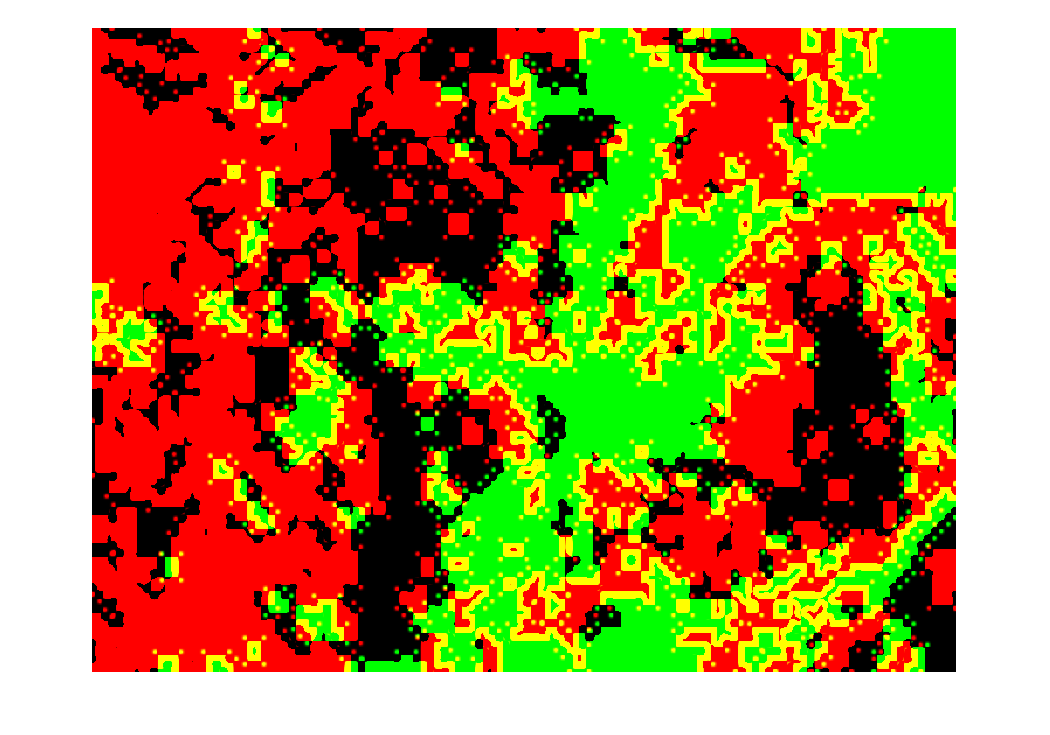
\includegraphics[width=\linewidth]{stride10im1.png}
  \caption{sliding window stride=10}\label{fig: sliding window problem}
\endminipage\hfill
\minipage{0.5\textwidth}
  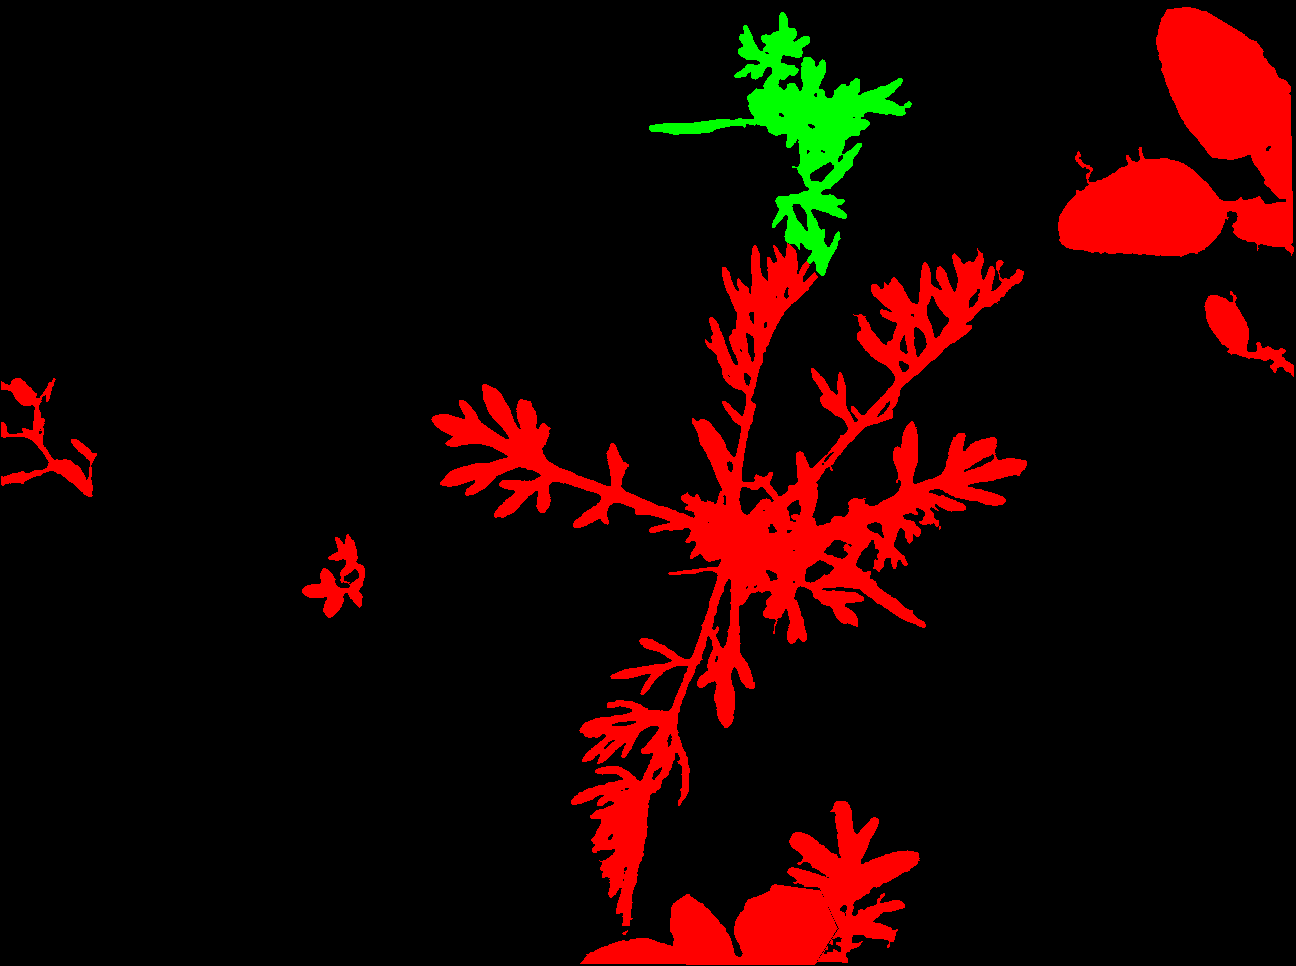
\includegraphics[width=\linewidth]{annotation.png}
  \caption{annotation}\label{fig:annotation}
\endminipage\hfill
\end{figure}
\newpage

\section{Umbalanced class problem}

The problem was that the network suffers of umbalanced data. Umbalanced data typically refers to a problem of classification where the classes are not represented equally. In fact what I have done was to count the pixels of crop, weed and ground from the annotation images referring to the training set and I discovered that:

\begin{itemize}

	\item \textbf{92,50\%} of the pixels are marked as ground
	\item \textbf{5,96\%} of the pixels are marked as weed
	\item \textbf{1,54\%} of the pixels are marked as crop

\end{itemize}

I tried to solve this problem by apply a threshold on the probabilities results of the ground patches. The threshold must be a value for which the 92,50\% of the ground probability are bigger.In other words:

\begin{center}
	$ T = groundVector[numberOfPatches\times 0,9250] $
\end{center}

where $groundVector $ is the vector containing the probabilities of the ground patches in descending order and $numberOfPatches $ is the number of patches apply to the image.\\
What I get was that the results looks better with an accuracy close to $ 70\% $ but the networks failed to classify crop form weed. So I decided to apply the same threshold approach also for the crop probabilities and what I get are an overall accuracy from all the test images of 89,62\% for a stride of 10 and 91,25\% for a stride of 15.\\
Here are some results. The full results can be view in the gitHub repository\footnote{see Appendix Repository}.

\begin{figure}[!htb]
\minipage{0.6\textwidth}
  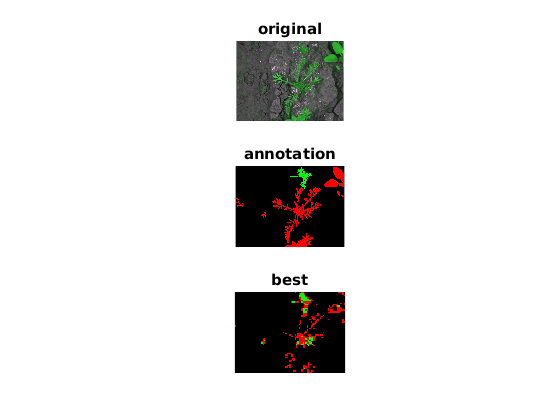
\includegraphics[width=\linewidth]{1.png}
  \caption{sliding window stride=15}\label{fig: sliding window 15 1}
\endminipage\hfill
\minipage{0.6\textwidth}
  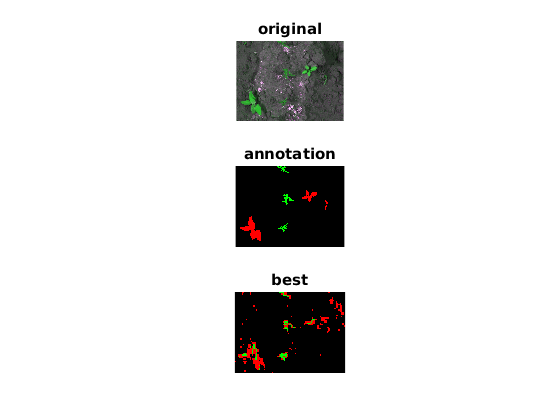
\includegraphics[width=\linewidth]{3.png}
  \caption{sliding window stride=15}\label{fig:sliding window 15 2}
\endminipage\hfill
\end{figure}

\begin{figure}[!htb]
\minipage{0.6\textwidth}
  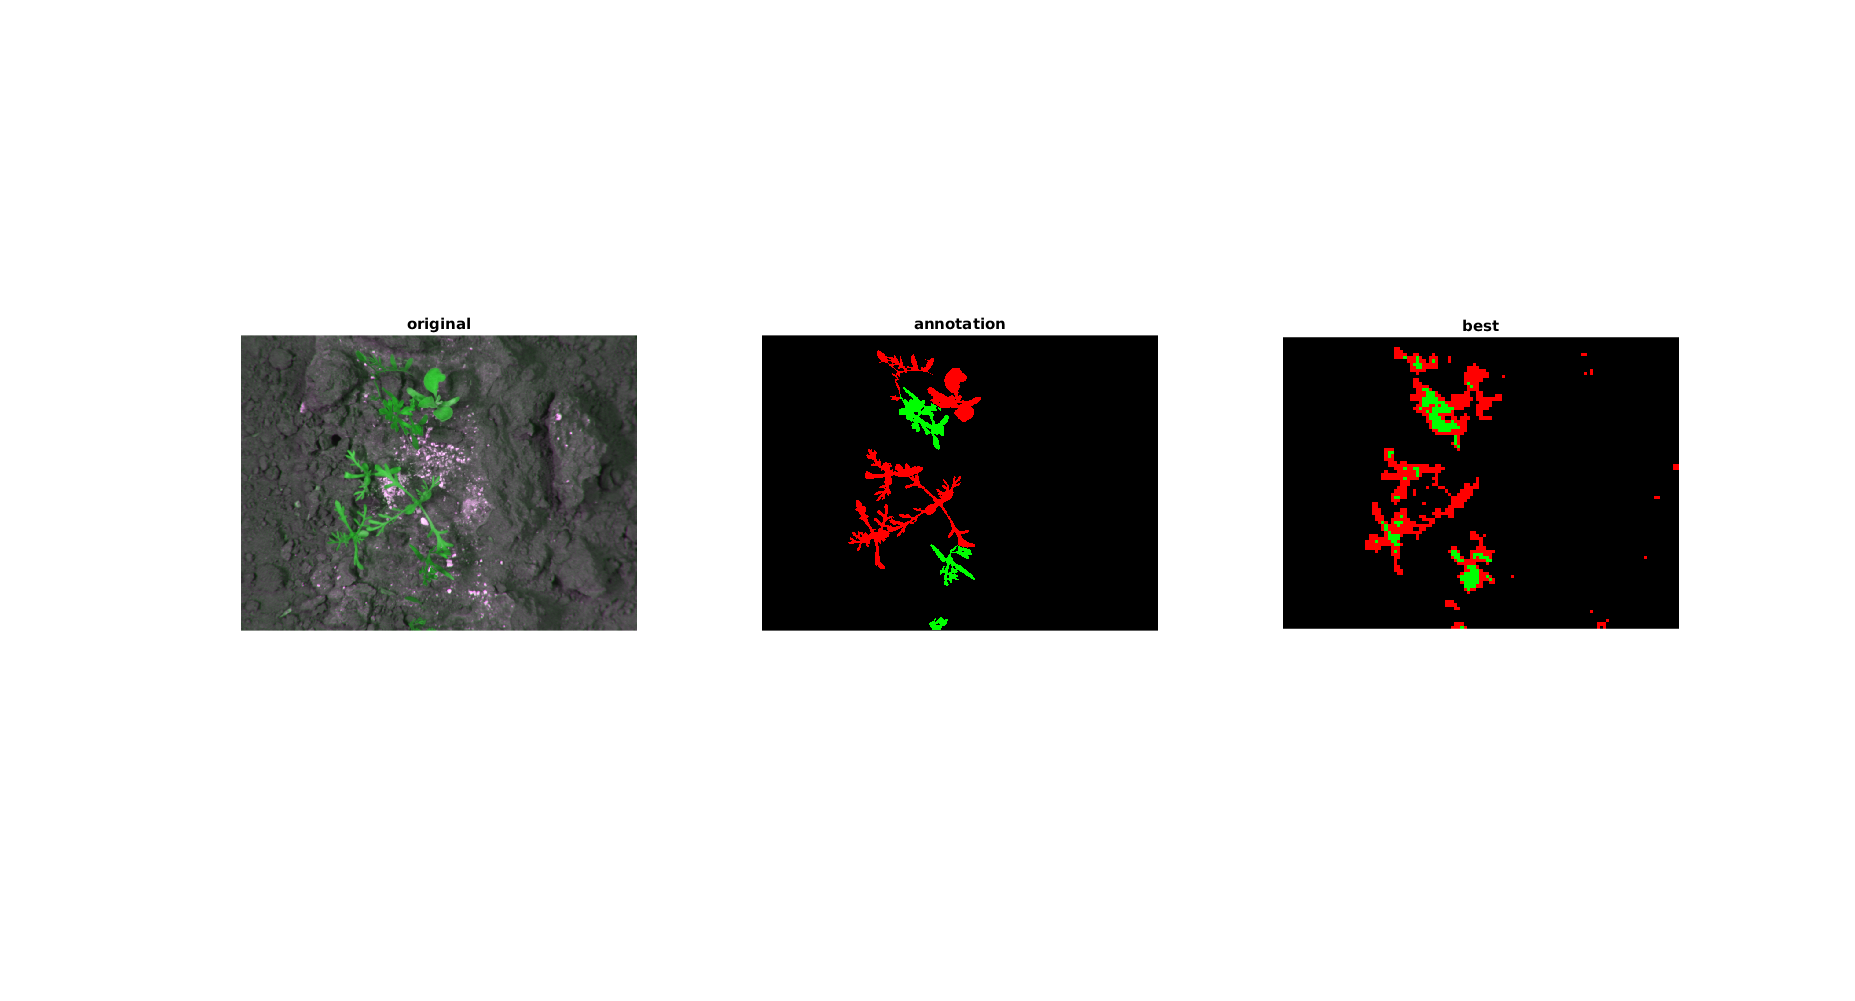
\includegraphics[width=\linewidth]{2.png}
  \caption{sliding window stride=10}\label{fig: sliding window 10 1}
\endminipage\hfill
\minipage{0.6\textwidth}
  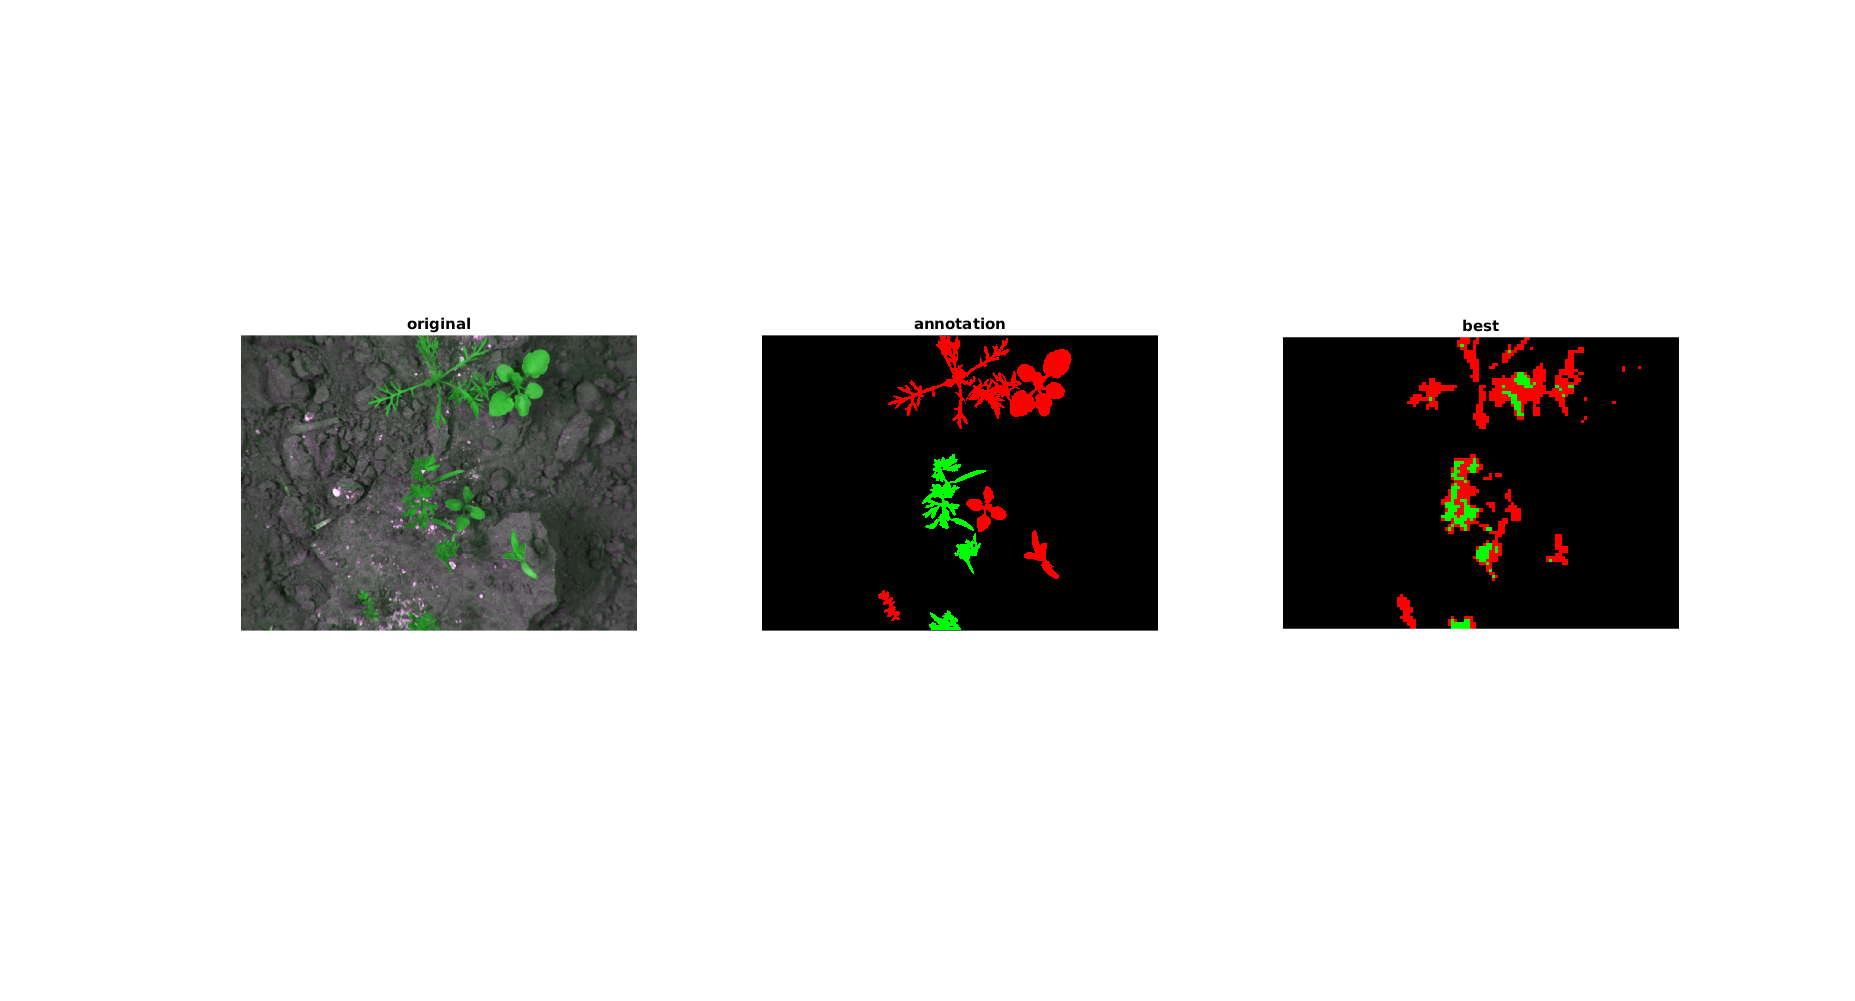
\includegraphics[width=\linewidth]{6.png}
  \caption{sliding window stride=10}\label{fig:sliding window 10 2}
\endminipage\hfill
\end{figure}


\chapter{Summary and future extensions}

In this chapter I want to make some considerations about how the network works and some future extensions that can be applied in order to have a better performance of the network.
If we look at the result of the sliding window we can see that in some images the network classifies some crop pixel as weed. This wrong classifications are due to the threshold approach applied in the section 4.5. In fact, if in the image there are more crop pixels than the one that I calculate in the training set (1,54\%) the network classifies only few pixels as crop. Below I attached an image that shows this behaviour of the network.

\begin{figure}[h]
	\begin{center}
		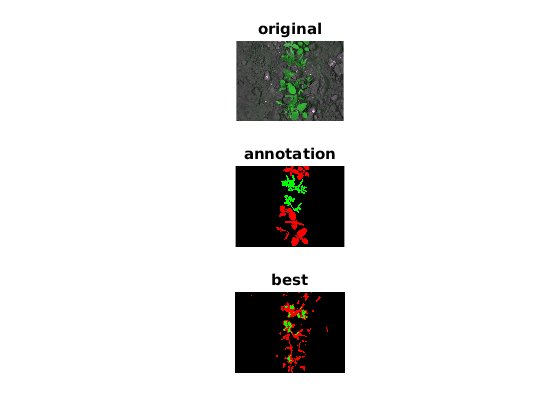
\includegraphics[scale=0.62]{15.png}
		\caption{bad sliding window result}
		\label{fig:bad sliding window result}
	\end{center}
\end{figure}
\newpage

The result show that a lot of crop pixels are marked as weed and also a lot of weed pixels are marked as ground (the percentage of weed pixels in the training set was 5,96\%).

\section{Possible extensions}

In order to have a better performance of the network some solution and extensions can be done:

\begin{itemize}

	\item \textbf{have a larger dataset}: if we have more patches the network could possibly work 			          better. In order to have more patches rotation could be applied
	
	\item \textbf{resampling the dataset}: 
   \begin{enumerate}
   
		\item we can add copies of instances from the under-represented class called over-		              sampling,or more formally sampling with replacement
		\item we can delete instances from the over-represented class, called under-sampling
   
   \end{enumerate}
   
   \item \textbf{try penalized models}: we can use the same algorithms but give them a different perspective on the problem.
Penalized classification imposes an additional cost on the model for making classification mistakes on the minority class during training. These penalties can bias the model to pay more attention to the minority class 

\end{itemize}

\chapter{Appendix}

\section{Repository}

All the code, the dataset, the intermediate results and other documents can be found at this repository \url{https://github.com/ste93ste/cwfid_classification}

\section{Reference document}
 \begin{itemize}
 
 	\item\url{http://rd.springer.com/chapter/10.1007%2F978-3-319-16220-1_8}
	
 \end{itemize}

\section{Software and tool used}

\begin{itemize}
	
	\item LaTeX (\url{http://www.latex-project.org/}) : to redact and to format this document
	
	\item Matlab R2016a (\url{http://uk.mathworks.com/products/matlab/}) : to compute and 					  evaluate the network
	
	\item MatConvNet (\url{http://www.vlfeat.org/matconvnet/}) : MATLAB toolbox implementing 				  Convolutional Neural Networks (CNNs) 
	 
\end{itemize}

\end{document}          
